\documentclass[]{beamer}
\usepackage{beamerthemesplit} 
\usefonttheme{professionalfonts}
\usefonttheme{serif}
\usepackage{geometry}
\usepackage{graphicx}
\usepackage{amssymb}
\usepackage{ bm }
\usepackage{amsmath}
\usepackage{hyperref}
\usepackage{caption}
\usepackage{algorithm}
\usepackage[noend]{algorithmic}
\usepackage{tikz}
\usetikzlibrary{shapes,arrows,shadows}

\begin{document}

\title{Deep Q-Networks for Event Summarization}  
\author[Francisco Javier Arceo \& Chris Kedzie]
       {\parbox[t]{1.5in}{Francisco Javier Arceo \\ \href{mailto: fja2114@columbia.edu}{\color{blue} \small  fja2114@columbia.edu} } \and 
        \parbox[t]{1.5in}{Chris Kedzie \\  \and \href{mailto: kedzie@cs.columbia.edu}{\color{blue} \small kedzie@cs.columbia.edu} }}
        
\institute{ \large Columbia University in the City of New York}
\date{December 13, 2016}

\bibliographystyle{plain}

\begin{frame}
\titlepage
\end{frame}

\begin{frame}
	\frametitle{Agenda} 
	\tableofcontents
	
\end{frame}

% Slide 1

\section{Event Summarization}
	\subsection{Motivation}
\begin{frame}
	\frametitle{Event Summarization} 
	The primary goal of Event Summarization is to summarize an event over time.
	\begin{itemize}
	\item<2-> 	As crises unfold and many articles are generated about a given event, it is beneficial to have a meaningful summary about the incident. 
	\item<2-> Given the seemingly countless number of news and media outlets, reading and summarizing all of this content is impractical. 
	\item<2-> 	Instead, it is useful to have a system that evaluates these articles automatically and returns the most valuable information.
	\end{itemize}
\end{frame}
\begin{frame}
	\frametitle{Extractive Event Summarization} 
	We can structure this problem analytically and find methods to solve Event Summarization (or at least try to). 
	\begin{itemize}
	\item<2-> 	Extractive streaming summarization takes as input a short text description of a topic or an event known as a query, a document stream, and a time ordered set of sentences relevant to the query. 
	\item<2-> The algorithm sequentially examines each sentence from the document stream and includes the candidate sentence into the summary when novel and important information is detected. 
	\end{itemize}
\end{frame}


\begin{frame}
	\frametitle{Previous Work in Extractive Event Summarization} 
	\begin{itemize}
		\item<1-> Recent research in text retrieval  has focused on extractive algorithms to identify important sentences from a large set of documents for summarizing articles from different events in the news (e.g., \cite{diazquery}, \cite{kedzie2015predicting}, \cite{garbacea2015university}, and \cite{kedzieextractive}).
		\item<1-> \cite{kedzie2015predicting}  has shown that it is possible to select relevant sentences from a massive number of documents on the web to create summaries with meaningful content by adapting classifiers to maximize search policies.
		\item<1-> These systems have been shown to  fall short of simple heuristic algorithms \cite{garbacea2015university}, which may be due to the limited ability of traditional n-gram models to capture the rich and often idiosyncratic structure of language.
	\end{itemize}

\end{frame}

\begin{frame}
	\frametitle{Deep Q-Networks for Event Summarization} 
This leads us to explore Deep Q-Networks (DQN) for 3 reasons: 
	 \vspace{-0.2cm} \begin{enumerate}
	\item <1-> We can define an architecture that propagates information end-to-end about the inputs, actions, and rewards 
	\item <1-> The representation and interaction between the stream, summary, and query can be learned jointly
	\item <1 -> RNN-LSTM embeddings can learn a more robust semantic representation than classical n-gram models
	\end{enumerate}
\end{frame}


\section{Deep Q-Networks}
	\subsection{Review}  
	\begin{frame}
			\frametitle{Deep Q-Networks: A Brief Introduction}
		\begin{itemize}
		\item <1 -> Q-Learning is a Reinforcement Learning framework that finds an optimal policy by taking an input state, set of possible actions available,  and returning the action with the highest reward.
		\item <1 -> When the state-action space becomes intractable, deterministic algorithms are no longer feasible for an optimal policy and researchers instead train a model to learn the policy. 
		\item <1 -> Deep Q-Networks \cite{MnihKSGAWR13} are an increasingly popular framework for learning these policies from end-to-end.
		\end{itemize}
	\end{frame}
	
	\subsection{DQN-LSTM}  
	\begin{frame}
		\frametitle{State, Action, and Rewards}
		\begin{itemize}
	\item<1 ->  The state $s(x_{t},\tilde{y}_{t}, d)$ at time $t$ is a function of the candidate sentence, $x_t$ to include in the summary, the state of the current summary $\tilde{y}_t$, and the query $d$. 	
	\item<1 -> The set of actions as $\mathcal{A} := \{select, skip\}$, which corresponds to
	\begin{equation}
		\tilde{y}_{t + 1} =
		\begin{cases}
			\tilde{y}_{t} \cup \{ x_t \},	& \text{if } a_t = select  \\
			\tilde{y}_{t}, 			& \text{if } a_t = skip.
		\end{cases}
	\end{equation}
	\item<1 -> The reward $r$ for a given action $a$ at time $t$ is measured by the change in ROUGE-F1 score of the predicted summary $\tilde{y}_{t}$ measured against a gold standard summary $Y$. 
	
		\end{itemize}
	\end{frame}

	\subsection{Actions}
	\begin{frame}
			\frametitle{Actions}
			We define our set of actions as $\mathcal{A} := \{select, skip\}$ where $select$ corresponds to adding the current sentence $x_t$ to the predicted summary $\tilde{y}_t$ and incrementing the current system time, or $skip$ where only $t$ is incremented without changing the current summary. Simply, 
			
	\begin{equation}
		\tilde{y}_{t + 1} =
		\begin{cases}
			\tilde{y}_{t} \cup \{ x_t \},	& \text{if } a_t = select  \\
			\tilde{y}_{t}, 			& \text{if } a_t = skip.
		\end{cases}
	\end{equation}

	\end{frame}

	\subsection{Rewards}
	\begin{frame}
			\frametitle{Reward}
				The reward $r$ for a given action $a$ at time $t$ is measured by the change in ROUGE-F1 score of the predicted summary $\tilde{y}_{t}$ measured against a gold standard summary $Y$. 
	\begin{equation}
		 \textrm{ROUGE-R}(\tilde{y}, Y) = 
		    \frac{\sum_{g \in Y} 
		    \min \left(\textrm{count}(g, \tilde{y}), \textrm{count}(g, Y)\right)}{
		    \sum_{g \in Y} 
		    \textrm{count}(g, Y)
	    }
	\end{equation}
	\begin{equation}
		 \textrm{ROUGE-P}(\tilde{y}, Y) = 
		    \frac{\sum_{g \in \tilde{Y}} 
		    \min \left(\textrm{count}(g, \tilde{y}), \textrm{count}(g, Y)\right)}{
		    \sum_{g \in \tilde{Y}} 
		    \textrm{count}(g, \tilde{Y})
	    }
	\end{equation}
				\begin{equation}
					r_t = \textrm{ROUGE-F1}(\tilde{y}_{t}, Y) -  \textrm{ROUGE-F1}(\tilde{y}_{t-1}, Y).
				\end{equation}
	\end{frame}

	\subsection{Policy}
	\begin{frame}
			\frametitle{Policy}
			\begin{itemize}
				\item<1-> We define our Q-Learner as an RNN-LSTM that is trained by randomly exploring the state-space using an $\epsilon$-greedy search over actions and states. 
				\item<1->We train our Q-Learner by iteratively updating the learned extraction policy through backpropagation of the observed reward for each action.
				\item<1-> We define an architecture similar to that of \cite{narasimhan2015language} and map our three inputs (query, sentence, and current predicted summary) into LSTM embeddings according to $\textbf{Figure 1}$
			\end{itemize}
	\end{frame}
\begin{frame}
\begin{center}
	\frametitle{Architecture of the Q-Learner}
    \pgfdeclarelayer{background}
    \pgfdeclarelayer{foreground}
    \pgfsetlayers{background,main,foreground}
        % Define the layers to draw the diagram
        \tikzstyle{sensor}=[draw, fill=blue!10, text width=5em,  text centered, minimum height=2.0em,drop shadow]
        \tikzstyle{term}=[draw, fill=gray!10, text width=5em,  text centered, minimum height=2.0em,drop shadow]
        \tikzstyle{wa} = [sensor, fill=gray!10, text width=5em,  minimum height=2em, rounded corners, drop shadow]
        \tikzstyle{wa} = [sensor, fill=gray!10, text width=5em,  minimum height=2em, rounded corners, drop shadow]
        \tikzstyle{wa2} = [sensor, fill=gray!10, text width=6em,  minimum height=12em, drop shadow]
        \tikzstyle{om} = [draw, fill=green!05, text width=6em,  text centered, minimum height=2.0em,drop shadow]

    \begin{tikzpicture}[scale=0.6, transform shape]
            \node (wa) [wa2] {Joined \textbf{ReLU Layer}  \\ \scriptsize (3 x Embedding) };
            \path (wa.west)+(-3.0 ,  2.0) node (asr1)[sensor] { $Query$ \textbf{LSTM}};
            \path (wa.west)+(-3.0 ,  0.0) node (asr2)[sensor] {$Sentence_t$  \textbf{LSTM}};
            \path (wa.west)+(-3.0 , -2.0) node (asr3)[sensor] {$Summary_t$  \textbf{LSTM}};
            \path (wa.east)+(3.0,  1) node (vote) [term] {\textbf{Linear} \\ \scriptsize $\{Rouge, Select\}$ };
            \path (wa.east)+(3.0, -1) node (vote2) [term] {\textbf{Linear} \\ \scriptsize $\{Rouge, Skip\}$ } ;
            \path (wa.east)+(6.5,  0) node (output) [om] {\textbf{Linear} \\ \scriptsize E[Rouge ,$a_t$]} ;

            \path [draw, ->] (asr1.east) -- node [above] {}     (wa.125);
            \path [draw, ->] (asr2.east) -- node [above] {}     (wa.180);
            \path [draw, ->] (asr3.east) -- node [above] {}     (wa.235);
            \path [draw, ->] (wa.east) -- node [above] {}       (vote.west);
            \path [draw, ->] (wa.east) -- node [above] {}       (vote2.west);
            \path [draw, ->] (vote.east) -- node [above] {}     (output.175);
            \path [draw, ->] (vote2.east) -- node [above] {}   (output.185);

         \begin{pgfonlayer}{background}[transparency group,opacity=.5]
                \path (asr1.north  |- asr1.south)+(-2.0, 1.6) node (a) {};
                \path (asr3.west  |- vote.east)+(+10.0, -3.5) node (b) {};
                \path (asr3.west  |- vote.east)+(+10.0, -2.5) node (c) {};
                \path (asr3.east  |- output.east)+(+13, -4.50) node (d) {};
                \path[fill=white!20,rounded corners, draw=black!100, dashed]         (a) rectangle (d);
            \end{pgfonlayer}

         \begin{pgfonlayer}{background}[transparency group,opacity=.5]
                \path (asr1.north  |- asr1.south)+(-1.7, 1.3) node (a) {};
                \path (asr3.west  |- asr3.east)+(+10.0, -3.5) node (b) {};
                \path (asr3.west  |- asr3.east)+(+10.0, -2.5) node (c) {};
                \path (asr3.west  |- asr3.east)+(+2.9, -1.50) node (d) {};
                \path[fill=white!20,rounded corners, draw=blue!100, dashed]         (a) rectangle (d);
            \end{pgfonlayer}

         \begin{pgfonlayer}{background}[transparency group,opacity=.5]
                \path (asr1.north  |- asr1.south)+(2.7, 1.3) node (a) {};
                \path (asr3.west  |- asr3.east)+(+10.0, -3.5) node (b) {};
                \path (asr3.west  |- asr3.east)+(+10.0, -2.5) node (c) {};
                \path (asr3.west  |- asr3.east)+(+11.5, -1.50) node (d) {};
                \path[fill=white!20,rounded corners, draw=gray!100, dashed]         (a) rectangle (d);
            \end{pgfonlayer}

         \begin{pgfonlayer}{background}[transparency group,opacity=.5]
                \path (asr1.north  |- asr1.south)+(7.4, 1.0) node (a) {};
                \path (asr3.west  |- asr3.east)+(+10.0, -3.5) node (b) {};
                \path (asr3.west  |- asr3.east)+(+10.0, -2.5) node (c) {};
                \path (asr3.west  |- asr3.east)+(+11.3, -0.50) node (d) {};
                \path[fill=red!05,rounded corners, draw=black!100, dashed]         (a) rectangle (d);
            \end{pgfonlayer}

         \begin{pgfonlayer}{background}[transparency group,opacity=.5]
                \path (asr1.north  |- asr1.south)+(10.7, 1.3) node (a) {};
                \path (asr3.west  |- asr3.east)+(+10.0, -3.5) node (b) {};
                \path (asr3.west  |- asr3.east)+(+10.0, -2.5) node (c) {};
                \path (asr3.west  |- asr3.east)+(+15.1, -1.50) node (d) {};
                \path[fill=white!20,rounded corners, draw=green!100, dashed]         (a) rectangle (d);
            \end{pgfonlayer}

            \path (wa.west) + (5.8,    2.25)  node (vote.east) {\scriptsize \textbf{Action} }; 
%            \path (wa.west) + (5.8,    1.95)  node (vote.east) {\scriptsize $\{argmax(a_t)$\}}; 
            \path (wa.west) + (-2.90, -3.2)  node (vote.east) {Input}; 
            \path (wa.west) + (3.5,    -3.2)  node (vote.east) {State-Action Representation }; 
            \path (wa.west) + (9.30,  -3.2)  node (vote.east) {Output};
            \path (wa.east) + (0.5, -4.2)  node (vote.east) {\textbf{Figure 1: DQN-LSTM Architecture}};
    \end{tikzpicture}
    \end{center}
    \vspace{-0.2cm} \tiny *ReLU(x) = max(0, x)
\end{frame}


\subsection{Algorithm}
	\begin{frame}
			\frametitle{Overview of Algorithm}
			DQN-LSTM for Event Summarization Training Procedure
			\begin{center}
			  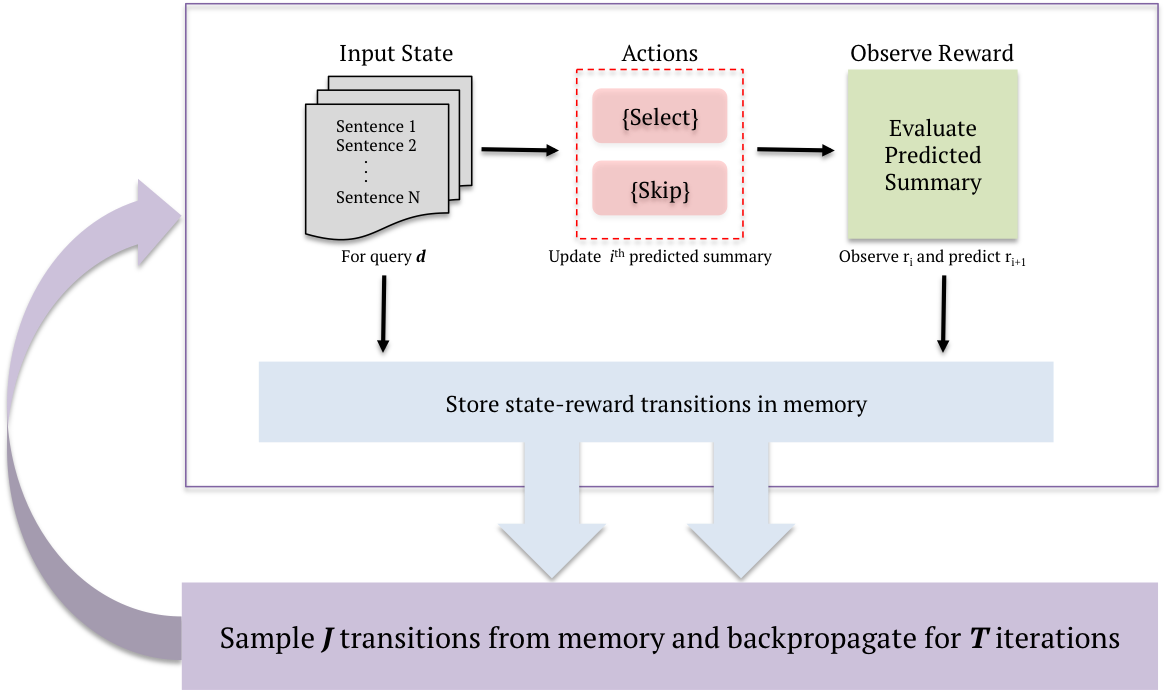
\includegraphics[scale=0.45]{DQN_LSTM_Algorithm}
			\end{center}
	\end{frame}

\begin{frame}
\begin{algorithm}[H]
  \algsetup{linenosize=\tiny}
  \tiny
        \textbf{Input:} { \rm  \{$\mathcal{D}$: Event queries, $X_d$: Input sentences, $N$: Number of epochs\} } \\
        \underline{\textbf{Output:} \rm \{$\hat{Q}$: extraction policy, $\tilde{Y}_d$: event summary for query $d$\} }
\begin{algorithmic}[1]
    \STATE \rm Initialize extraction policy $\hat{Q}$ with random weights
    \STATE \rm Initialize memory and summary: $\Gamma, \tilde{Y} =  \{\emptyset \}^{\mathcal{|D|}}_{d=1},  \{\emptyset \}^{\mathcal{|D|}}_{d=1} $
    \FOR{$epoch=1,..,N\ $}
        \FOR{query $d \in \mathcal{D}$}
            \STATE $X_{d}, \tilde{Y}_{d}$ = \{Extract $t=1,...,T_d$ ($sentences_d$, $summary_d$)\}
            \FOR{$x_t, \tilde{y}_t \in X_d, \tilde{Y}_d$ }
                \STATE Set $s_t = s(x_t, \tilde{y}_t, d)$
                \STATE $ \forall a_t \in \mathcal{A}(s_t)$ \textrm{compute} $\hat{Q}(s_t, a_t)$ and select $a^{*}_t =$ argmax$_{a_{t}}\hat{Q}(s_t, a_t)$
                \STATE  \textbf{if} $random() < \epsilon$ \textbf{then} select $a^{*}_t $ at random with $\Pr(a_t) =\frac{1}{| \mathcal{A} |} $
                \STATE Update $\tilde{y}_{t+1}$ according to equation (1)
                \STATE Execute action $a^{*}_t$ and observe reward $r_t$ and new state $s_{t+1}$
                \STATE Update $\Gamma_d = \Gamma_d \cup \{ [s_t, a^{*}_t, r_t, s_{t+1}]\}$
            \ENDFOR
        \ENDFOR
            \FOR{ $j=1,...,J$ transitions sampled from $\Gamma$}
                \STATE \[\textrm{Set } y_j =
                        \begin{cases}
                            r_j                                             & \text{if $s_{j+1}$ is terminal } \\
                                r_j + \gamma $max$_{a'}\hat{Q}(s_{j+1}, a'; \theta)     & \text{if $s_{j+1}$ is non-terminal } 
                        \end{cases} 
                        \]
                        \STATE Perform gradient step on $\mathcal{L}(\theta) = (y_j - \hat{Q}(s_j, a_j; \theta))^2$
            \ENDFOR
    \ENDFOR
\end{algorithmic}
\caption*{ DQN-LSTM for Event Summarization Training Procedure}
\label{alg:seq}
\end{algorithm}
\end{frame}

	
\section{Experiments}
	\subsection{Simulation}
		\begin{frame}
			\frametitle{Small Problems}
		Before evaluating the model on test data, it is illuminating to understand the in-sample training behavior of the architecture on a small-sample problem. Small sample experimentation allows us to
		\begin{enumerate}
		\item<1-> Verify that the model is able to solve our specified problem
		\item<1-> Understand the number of iterations required to explore the state-space
		\item<1-> Gain intuition about the impact of hyperparameters on the speed at which it takes to solve the problem
		\end{enumerate}
		\end{frame}

		\begin{frame}
			\frametitle{DQN-LSTM for 1 Query and 20 Sentences: Precision}
			Model learned to select the single best sentence.
			\begin{center}
			\framebox{
			  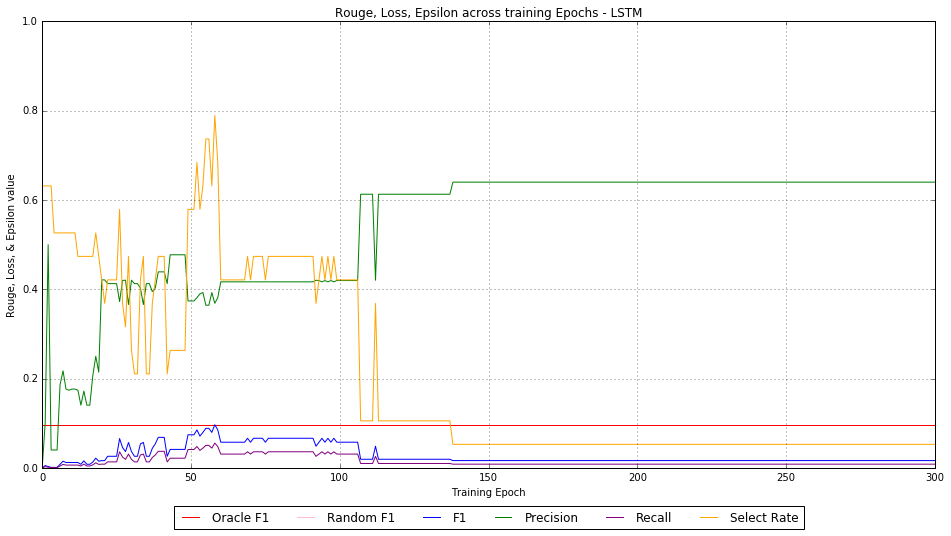
\includegraphics[height=2.0in,width=4.0in]{DQN_LSTM_Precision}
				}
			\end{center}
		\end{frame}
		
		\begin{frame}
			\frametitle{DQN-LSTM for 1 Query and 20 Sentences: Recall}
			Model learned to select all sentences.
			\begin{center}
			\framebox{
			  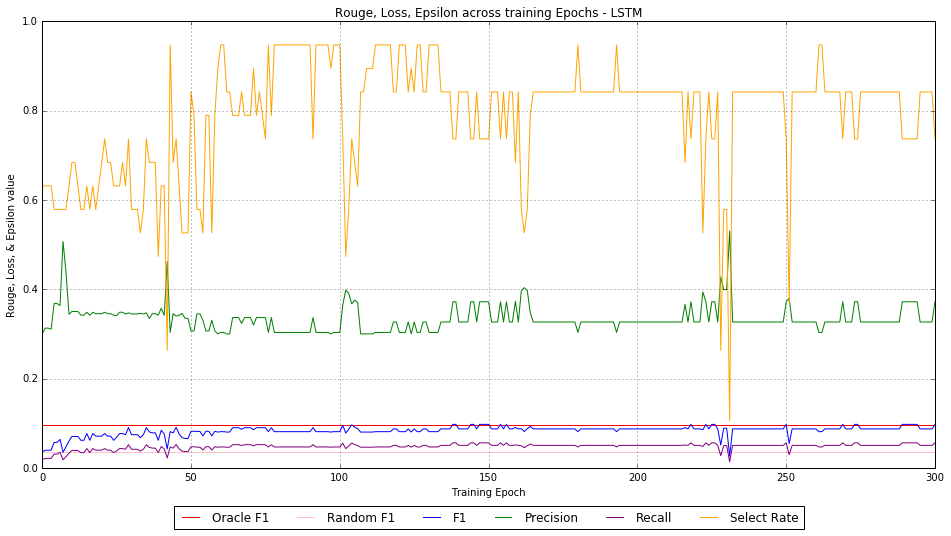
\includegraphics[height=2.0in,width=4.0in]{DQN_LSTM_Recall}
				}
			\end{center}
		\end{frame}
	
		\begin{frame}
			Model was able to maximize F1.
			\frametitle{DQN-LSTM for 1 Query and 20 Sentences: F1}
			\begin{center}
			\framebox{
			  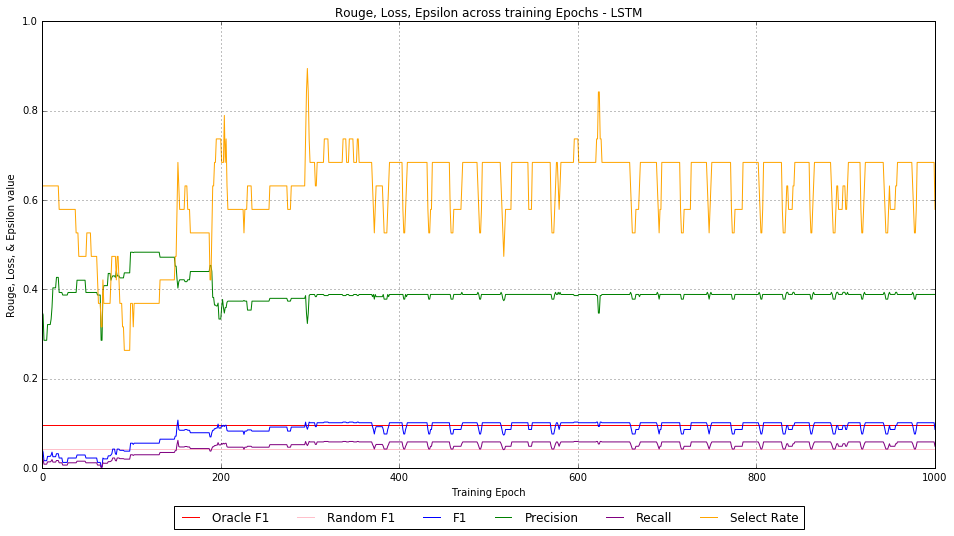
\includegraphics[height=2.0in,width=4.0in]{DQN_LSTM_F1}
				}
			\end{center}
		\end{frame}

		\begin{frame}
			\frametitle{What did we learn?}
			The experiments are extremely useful in understanding the implications of the specification of the network. We found that 
			\begin{center}
				\begin{enumerate}
					\item<1-> Maximizing Precision is easier than maximizing Recall.
					\item<1-> Choosing either Precision or Recall yields obvious pathological results; i.e., selecting the single best sentence or selecting all sentences.
					\item<1-> Optimizing F1 requires much longer training to choose the optimal strategy.
				\end{enumerate}
			\end{center}
		\end{frame}

%	\subsection{Benchmarking}
%		\begin{frame}
%			\frametitle{Evaluation}
%			\begin{itemize}
%		\item<1-> We benchmark our model against (1) an Oracle that greedily chooses to include sentences if the increase in ROUGUE-F1 is positive,  (2) random selection of sentences,  and (3) a bag-of-words multilayer perceptron.
%		\item<1-> We use n-fold cross validation and average the F1 across the held-out test queries.
%		\end{itemize}
%	\end{frame}



\section{Resources}
\begin{frame}
	\frametitle{References and Links}
	Thank you
	\begin{itemize}
	\item<1-> \color{blue} \href{https://github.com/franciscojavierarceo/DQN-Event-Summarization}{GitHub Repository}
	\end{itemize}
\end{frame}

\bibliography{DQN-Event-Summarization}

\end{document}